\def\layersep{1cm}
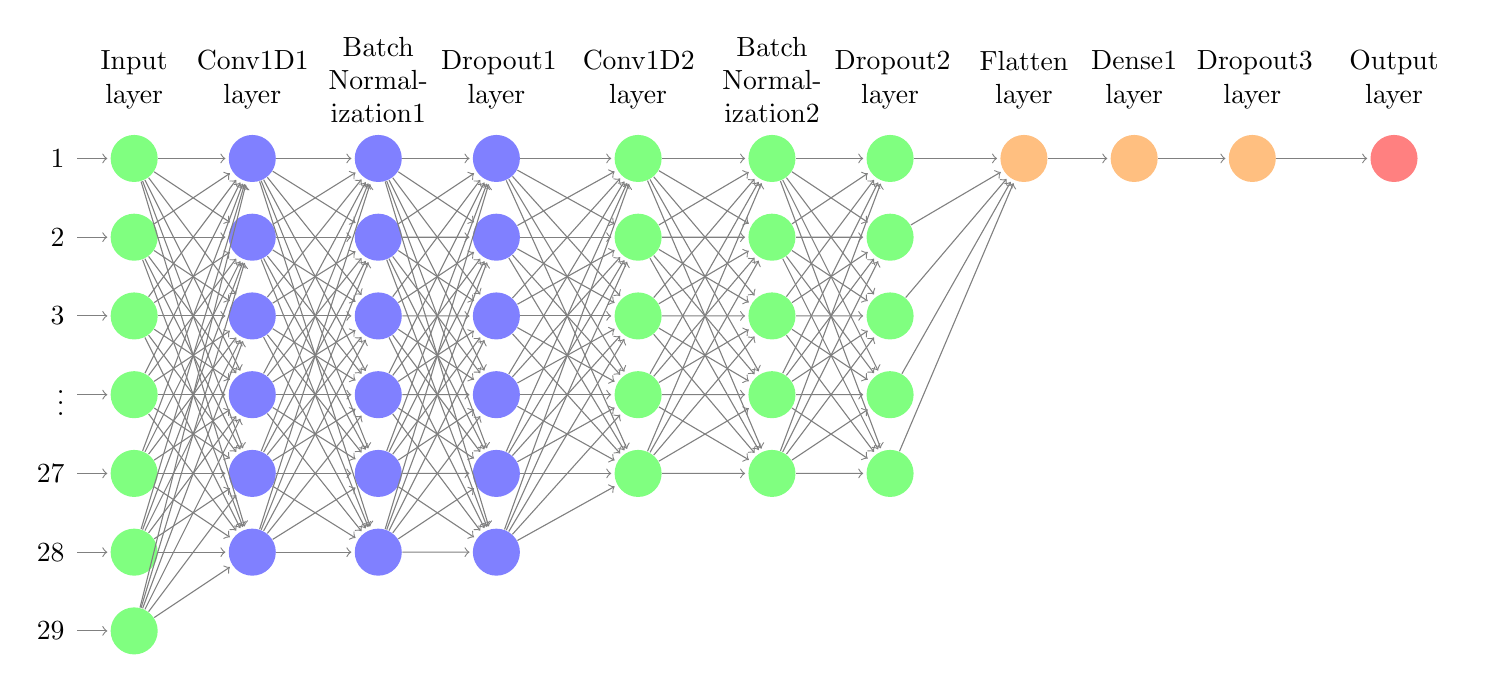
\begin{tikzpicture}[shorten >=1pt,->,draw=black!50, node distance=\layersep]
	\tikzstyle{every pin edge}=[<-,shorten <=1pt]
	\tikzstyle{neuron}=[circle,fill=black!25,minimum size=17pt,inner sep=0pt]
	\tikzstyle{input neuron}=[neuron, fill=green!50];
	\tikzstyle{fase1 neuron}=[neuron, fill=blue!50];
	\tikzstyle{fase2 neuron}=[neuron, fill=green!50];
	\tikzstyle{fase3 neuron}=[neuron, fill=orange!50];
	\tikzstyle{output neuron}=[neuron, fill=red!50];
	\tikzstyle{annot} = [text width=4em, text centered]
	
	% Draw the input layer nodes
	\foreach \y in {1,...,7}{
		% This is the same as writing \foreach \name / \y in {1/1,2/2,3/3,4/4}
		\ifnum\y<4
		\node[input neuron, pin=left: \y] (I-\y) at (0,-\y) {};
		\fi
		\ifnum\y=4
		\node[input neuron, pin=left: \vdots] (I-\y) at (0,-\y) {};
		\fi
		\ifnum\y=5
		\node[input neuron, pin=left: 27] (I-\y) at (0,-\y) {};
		\fi
		\ifnum\y=6
		\node[input neuron, pin=left: 28] (I-\y) at (0,-\y) {};
		\fi
		\ifnum\y=7
		\node[input neuron, pin=left: 29] (I-\y) at (0,-\y) {};
		\fi
	}
	
	% Draw the Conv1D_1 nodes
	\foreach \y in {1,...,6}
	\node[fase1 neuron, right of=I-4] (H1-\y) at (\layersep*0.5,-\y) {};
	
	% Draw the Batch_Normalization_1 nodes
	\foreach \y in {1,...,6}
	\node[fase1 neuron, right of=H1-4] (H2-\y) at (\layersep*2.1,-\y) {};
	
	% Draw the Dropout_1 layer nodes
	\foreach \y in {1,...,6}
	\node[fase1 neuron, right of=H2-4] (H3-\y) at (\layersep*3.6,-\y cm) {};
	
	% Draw the Conv1D_2 nodes
	\foreach \y in {1,...,5}
	\node[fase2 neuron, right of=H3-4] (H4-\y) at (\layersep*5.4,-\y cm) {};
	
	% Draw the Batch_Normalization_2 nodes
	\foreach \y in {1,...,5}
	\node[fase2 neuron, right of=H4-4] (H5-\y) at (\layersep*7.1,-\y) {};
	
	% Draw the Dropout_2 layer nodes
	\foreach \y in {1,...,5}
	\node[fase2 neuron, right of=H5-4] (H6-\y) at (\layersep*8.6,-\y cm) {};
	
	% Draw the Flatten layer nodes
	\node[fase3 neuron, right of=H6-4] (H7-1) at (\layersep*10.3,-1 cm) {};
	
	% Draw the Dense_1 layer nodes
	\node[fase3 neuron, right of=H7-1] (H8-1) at (\layersep*11.7,-1 cm) {};
	
	% Draw the Dropout_3 layer nodes
	\node[fase3 neuron, right of=H8-1] (H9-1) at (\layersep*13.2,-1 cm) {};
	
	% Draw the Dense_2 layer nodes
	\node[output neuron, right of=H9-1] (H10-1) at (\layersep*15,-1 cm) {};
	
	% Connect every node in the input layer with every node in the
	% Conv1D_2 layer.
	\foreach \source in {1,...,7}
	\foreach \dest in {1,...,6}
	\path (I-\source) edge (H1-\dest);
	% Connect every node in the Conv1D_2 layer with every node in the
	% Batch_Normalization_1 layer.
	\foreach \source in {1,...,6}
	\foreach \dest in {1,...,6}
	\path (H1-\source) edge (H2-\dest);
	% Connect every node in the Batch_Normalization_1 layer with every node in the
	% Dropout_1 layer.
	\foreach \source in {1,...,6}
	\foreach \dest in {1,...,6}
	\path (H2-\source) edge (H3-\dest);
	% Connect every node in the Dropout_1 layer with every node in the
	% Conv1D_2 layer.
	\foreach \source in {1,...,6}
	\foreach \dest in {1,...,5}
	\path (H3-\source) edge (H4-\dest);
	% Connect every node in the Conv1D_2 layer with every node in the
	% Batch_Normalization_1 layer.
	\foreach \source in {1,...,5}
	\foreach \dest in {1,...,5}
	\path (H4-\source) edge (H5-\dest);
	% Connect every node in the Batch_Normalization_1 layer with every node in the
	% Dropout_2 layer.
	\foreach \source in {1,...,5}
	\foreach \dest in {1,...,5}
	\path (H5-\source) edge (H6-\dest);
	% Connect every node in the Dropout_2 layer with every node in the
	% Flatten layer.
	\foreach \source in {1,...,5}
	\path (H6-\source) edge (H7-1);
	% Connect every node in the Flatten layer with every node in the
	% Dense_1 layer.
	\path (H7-1) edge (H8-1);
	% Connect every node in the Dense_1 layer with every node in the
	% Dropout_3 layer.
	\path (H8-1) edge (H9-1);
	% Connect every node in the Dropout_3 layer with every node in the
	% Dense_2 layer.
	\path (H9-1) edge (H10-1);
	
	% Annotate the layers
	\node[annot,above of=H1-1, node distance=1cm] {Conv1D1 layer};
	\node[annot,above of=H2-1, node distance=1cm] {Batch Normalization1};
	\node[annot,above of=H3-1, node distance=1cm] {Dropout1 layer};
	\node[annot,above of=H4-1, node distance=1cm] {Conv1D2 layer};
	\node[annot,above of=H5-1, node distance=1cm] {Batch Normalization2};
	\node[annot,above of=H6-1, node distance=1cm] {Dropout2 layer};
	\node[annot,above of=H7-1, node distance=1cm] {Flatten layer};
	\node[annot,above of=H8-1, node distance=1cm] {Dense1 layer};
	\node[annot,above of=H9-1, node distance=1cm] {Dropout3 layer};
	\node[annot,above of=I-1] {Input layer};
	\node[annot,above of=H10-1] {Output layer};
	
\end{tikzpicture}